\documentclass[]{scrreprt}
\usepackage{amsmath,amsfonts,graphicx, hyperref}

\graphicspath{
{figures/}
}

\setcounter{secnumdepth}{3}

\begin{document}


\title{Strata deformation above a longwall coal mine}
\author{CSIRO}
\maketitle

\tableofcontents

%%%
\chapter{Introduction}
%%%

In an underground longwall coal mine, coal is mined in ``panels'', as
shown in Figure~\ref{lw_mining_graphic.fig}.  These panels are typically 3--4\,m in
height, 150--400\,m in width and 1000--4000\,m long.  Coal is
extracted from one end, moving towards the other end.  As mining
progresses, a void is created behind the mining
machinery where the coal used to be.  The rock material above this
void --- the ``overburden'' -- is not strong enough to support itself,
so it collapses downwards.  The resulting partial void and collapsed
material is called the ``goaf'' (or ``gob'').

\begin{figure}[htb]
\begin{center}
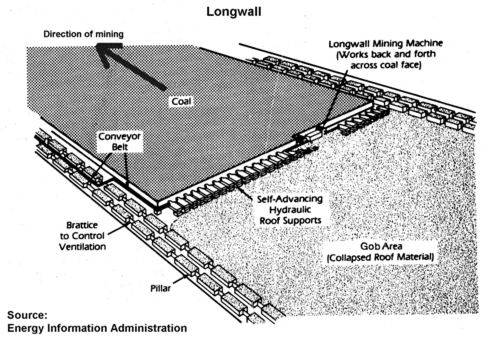
\includegraphics[width=10cm]{lw_mining_graphic.pdf}
\caption{Pictorial representation of a single panel in longwall
  mining.  The dimensions and process are described in the text.  Figure sourced from
  citizensagainstlongwallmining.org who obtained it from the Energy
  Information Administration.}
\label{lw_mining_graphic.fig}
\end{center}
\end{figure}

There are many geotechnical aspects that are of interest in this
process, but this Example concentrates on the following.
\begin{enumerate}
\item The vertical displacement of the ground surface due to the
  longwall mining.  This is called the ``subsidence''.  This obviously
  has effects on buildings and other man-made structures like roads,
  but it can also change surface water pathways, affect vegetation,
  and cause surface-water ponding, which all have effects on the local
  ecology.
\item\label{item2} The vertical deformation within the overburden.
\item The patterns of fracture in the overburden.  Together with
  Item~\ref{item2}, this can have effects on operational aspects of
  longwall mining, such as the load patterns on the ``chocks'' that
  support the roof of the goaf next to the mining machinery.  It also
  strongly effects the flow of fluids in the porous rocks that make up
  the overburden.  If the fracturing and deformation is extensive then
  fluids can easily move through the rock.  This can result in mines
  flooding with water, or causing excessive drawdown of groundwater
  aquifers which can effect other users of groundwater (such as
  irrigators for farming) or can effect the rates of groundwater
  baseflow to surrounding river systems which may effect local and
  not-so-local ecosystems.  The deformation and fracture of the
  overburden can also lead to aquifer mixing, where an aquifer
  consisting of ``dirty'' water (with high salinity, for example)
  pollutes a nearby aquifer of clean water.  The deformation and
  fracture can also lead to large releases of methane gas from
  overlying (and underlying) coal seams.  This methane can then flow
  through the highly permeable fractured rock system to the
  atmosphere, resulting in large greenhouse gas emissions.  Or it can
  flow to the mine workings which is extremely hazardous in terms of
  mine fires and explosions.
\end{enumerate}

This Example does not seek to build a realistic model of a specific
mine.  Instead, it explains how the TensorMechanics module can be used
to build such a model, by exploring a very simplified and contrived 2D
toy model, as well as a simple 3D model.  Of particular interest in
the 2D model are the input parameters used and how they effect the
results.

\chapter{The 2D model setup}
\label{m.d.chap}

\section{Geometry}

A 2D model representing a transverse section of overburden above a
longwall panel is primarily studied in this Example.  It is shown in
Figure~\ref{model_setup.fig}.  The longwall panel is 300\,m wide and the height of
extraction is 3\,m.  The transverse section describes only half
(150\,m) of the panel and it assumed that the situation is symmetric
about the panel's mid line.  The panel is 400\,m deep ($0\leq z\leq 400$).  The model
measures 450\,m in the $y$ direction ($0\leq y\leq 450$).  The model
is actually 1\,m in the $x$ direction but this is unimportant in the
subsequent analysis.

\begin{figure}[htb]
\begin{center}
\includegraphics[width=13cm]{model_seup.pdf}
\caption{A graphic of the 2D model used in this Example.  All
  dimensions are in metres.  The geometry is described in the text.}
\label{model_setup.fig}
\end{center}
\end{figure}

\section{Material properties}

The overburden is assumed homogeneous (but
anisotropic).  Boundary conditions are described below.  The
overburden's density is 2500\,kg.m$^{-3}$.

A number of different elasto-plastic models are used in the chapters
below, and their moduli are specified in those chapters.

\section{Boundary conditions}

All models use the following boundary conditions: roller on
$y_{\mathrm{min}}$ and $y_{\mathrm{max}}$; no rotation around the $x$
axis on $y_{\mathrm{min}}$; stress-free on the model's top; fixed
displacement on $z_{\mathrm{min}}$
where there is no excavation.

There are a number of different boundary conditions that may be
appropriate to use for the roof of the excavation.

\subsection{Roof: free}
\label{free.roof.sec}

The roof of the excavation is stress-free.  Therefore, the
overburden is free to move vertically under the action of gravity.
This simulates the case where there is no ``floor'' of the excavation.

\subsection{Prescribed roof displacements}
\label{prescribed.roof.defn.sec}

The free roof typically produces impossibly high displacements
because the floor of the excavation constrains
$u_{z}^{\mathrm{max}}\geq -3$\,m.  In fact, the floor strata ``heave''
--- they move slightly upwards --- so usually the maximum downwards
displacement might be between 2.5\,m and 2.9\,m in the case at hand.

A sophisticated approach for modelling the roof would be to use
MOOSE's Constrain system, but I have found that MOOSE's constraints
exhibit poor convergence in the case at hand.  An alternative option
is to prescribed displacements of the roof.  In this Example, the
prescribed boundary condition takes one of two forms:
\begin{eqnarray}
u_{z} & = & \left\{
\begin{array}{ll}
u_{z}^{\mathrm{max}} \max\left( \min\left( \left(
\frac{t}{t_{\mathrm{end}}}(y_{\mathrm{max}} - y_{\mathrm{min}}) +
y_{\mathrm{min}} - y \right) / d_{\mathrm{closure}}, 1 \right),
0\right) & \mbox{ or} \\
u_{z}^{\mathrm{max}} \frac{t}{t_{\mathrm{end}}} \max\left( \min\left(
(y_{\mathrm{max}} - y)/d_{\mathrm{closure}}, 1 \right), 0\right)
\end{array}
\right.
\end{eqnarray}
The following parameters are chosen: $u_{z}^{\mathrm{max}} = -3$\,m,
$y_{\mathrm{min}} = 0$, $y_{\mathrm{max}}=150$\,m and
$d_{\mathrm{closure}}=15$\,m.  These two forms correspond physically
to the following.
\begin{enumerate}
\item ``Sideways excavation'', where the coal is excavated from
  $y_{\mathrm{min}}$ to $y_{\mathrm{max}}$ during the time $0\leq
  t\leq t_{\mathrm{max}}$.  At time $t$, the excavation has reached $y_{t}
  = y_{\mathrm{min}} + t(y_{\mathrm{max}} -
    y_{\mathrm{min}})/t_{\mathrm{end}}$.  For $y$ less than this
    amount, the roof is allowed to displace a maximum
  of $u^{z}_{\mathrm{max}}$.  For $y$ greater than this amount, the
  roof has zero displacement.  There is a small region between
  $y_{t}-d_{\mathrm{closure}}$ and $y_{t}$ where the roof displacement
  is between zero and $u_{z}^{\mathrm{max}}$, but for
  $y<y_{t}-d_{\mathrm{closure}}$, $u = u_{z}^{\mathrm{max}}$.
\item ``Downwards excavation''.  The roof is gradually lowered.  At
  $t=0$ the displacement is zero, while at $t=t_{\mathrm{end}}$ the
  displacement is equal to $u_{z}^{\mathrm{max}}$ for most of the
  roof.  There is a small region between $y_{\mathrm{max}}$ and
  $y_{\mathrm{max}} - d_{\mathrm{closure}}$ where the displacement
  varies between zero and $u_{z}^{\mathrm{max}}$.
\end{enumerate}
A quasi-static solution is sought at each timestep, and no dynamics is
used, so ``time'' has no real physical meaning, except that it allows
the roof to be gradually lowered.

\subsection{Constrained roof}
\label{sitckybc.defn.}

Although MOOSE's full-blown Constraint system produces only very slow
convergence, TensorMechanics offers a ``StickyBC'' boundary condition
that may be used in the case at hand.  This boundary condition is: if
$u_{z}^{\mathrm{old}}<-3.0$\,m then fix $u_{z}$ forever more in the simulation.  This
does not allow for floor heave, otherwise the condition might be
$-2.5$\,m, for instance.  This type of boundary condition may only be
used in simulations with multiple excavation steps, since for just one
step $u^{\mathrm{old}}=0$ and the ``constrained roof'' boundary
condition becomes irrelevant.

In conjuction with this boundary condition, a time-varying Young's
modulus is used for the coal:
\begin{equation}
E = E_{\mathrm{full}}\max\left( \min\left( \left(
\frac{t}{t_{\mathrm{end}}}(y_{\mathrm{max}} - y_{\mathrm{min}}) +
y_{\mathrm{min}} - y \right) / d_{\mathrm{closure}}, 1 \right),
10^{-9} \right) \ .
\end{equation}
This simulates a ``sideways'' excavation, and enables the roof to
collapse under the overburden's weight.  The material with young's
modulus $E_{\mathrm{full}}\times 10^{-9}$ may be considered to be
mined and irrelevant to this Example.


\chapter{Elastic simulations with a free roof}
\label{elastic.chap}

The simulation results quoted in this section are derived using the
MOOSE input file {\tt cosserat\_elastic.i}.

\section{Motivation}

Setting the strata's yield strengths very high means that the
deformation is purely elastic.  Of course this is unphysical, but it
is interesting from a theoretical viewpoint.  An example deformation
is shown in Figure~\ref{cosserat_elastic_fig}.

The roof boundary condition is chosen to be ``free''
(Section~\ref{free.roof.sec}) to simplify the analysis.  This models
half of an excavation that is 300\,m wide.

\begin{figure}[htbp]
  \begin{center}
    \begin{tabular}{cc}
\multicolumn{2}{c}{\includegraphics[width=12cm]{cosserat_elastic_figure_1.pdf}} \\
      \includegraphics[width=6cm]{cosserat_elastic_figure_2.pdf} &
      \includegraphics[width=6cm]{cosserat_elastic_figure_3.pdf} \\
    \end{tabular}
\caption{Deformation of the overburden when using Cosserat elasticity
  with $T_{\mathrm{Cosserat}}=1$\,m and $k_{\mathrm{shear}}=1$\,GPa.m$^{-1}$.
  The bottom figures show ``subsidence'', which is vertical
  displacement on the top surface of the model; and ``extensometer''
  which is vertical displacement along a vertical line that runs down
  the left-hand-side of the mode.}
\label{cosserat_elastic_fig}
\end{center}
\end{figure}

\section{Beam theory}

The beam deformation may be compared with simple beam theory by
thinking of the overburden as a beam of thickness $T=400$\,m and
length $L=300$\,m, clamped at its ends and subject to its own self
load.  The maximum deflection of such a beam is
\begin{equation}
  u_{z}^{\mathrm{max}} = \frac{\rho TW g L^{4}}{384 EI} \ .
\end{equation}
Here $\rho=2500$\,kg.m$^{-3}$ is the beam's density, $W=10$\,m is its
width, $g=10$\,m.s$^{-2}$ is gravitational acceleration, $E=8$\,GPa is
the Young's modulus of the beam, $I$ its momenta of intertia:
\begin{equation}
  I = \int_{-T/2}^{T/2}{\mathrm d}z \int_{-W/2}^{W/2}{\mathrm d}x
  z^{2} = (2W/3)(T/2)^3 \ .
\end{equation}
Substituting this into the formula for maximum deflection yield
\begin{equation}
  u_{z}^{\mathrm{max}} = \frac{\rho g L^{4}}{32 ET^2} \approx
  800/T^{2} \ ,
  \label{eqn.elastic.delfection}
\end{equation}
(measured in units of m).
This formula will never give the precise displacement since various
assumptions (such as the pinned end conditions, and neglecting all but
the lowest-order terms) have been made in its
development.

\section{Comparison with beam theory --- non-Cosserat case}

Before
exploring the effects of introducing Cosserat mechanics, it is useful
to quantify the accuracy of Eqn~(\ref{eqn.elastic.delfection}) for
various $T$, using standard (non-Cosserat) elasticity (and modifying
the model described in Chapter~\ref{m.d.chap} to have an overburden of
thickness $T$ instead of just $T=400$\,m).    To do this,
the input file {\tt cosserat\_elastic.i} is used, but the layer
thickness, and Cosserat moduli are set very large.  The mesh used is
different in each case, but is set dense enough so that mesh
dependencies are small.

\begin{table}[htb]
\begin{center}
\begin{tabular}{cccc}
  T & Eqn~(\ref{eqn.elastic.delfection}) & MOOSE (non-Cosserat) & N \\
  \hline
  400 & 0.005 & 0.19 & 1000 \\
  100 & 0.08 & 0.33 & 1000 \\
  40 & 0.5 & 0.89 & 4000 \\
  10 & 8 & 8.7 & 20000\\
\end{tabular}
\caption{Comparison of the approximate analytic deflection of
  Eqn~(\ref{eqn.elastic.delfection}) with MOOSE's non-Cosserat
  result.  MOOSE's deflection is measured at the roof of the coal seam
  ($z=0$).  The last column, $N$, indicates the number of elements in
  the mesh before reasonable mesh-independence is obtained  ($N=1000$ was the
  minimum number tried).}
\label{elastic.deform.standard}
\end{center}
\end{table}

The results are tabulated in Table~\ref{elastic.deform.standard}.
Evidently, Eqn~(\ref{eqn.elastic.delfection}) under-predicts the
displacement for large $T$.  This is due to the extra freedom allowed
by the model compared with the pinned ends used by the theoretical
development, as well as higher-order terms that are obviously present
in such a thick beam.  Moreover, the MOOSE displacement is always a
function of $z$ (the vertical direction) as is obvious from
Figure~\ref{cosserat_elastic_fig}.

\section{Comparison with beam theory --- Cosserat case}

In many locations where coal seams are present, the overburden is
highly stratified: it consists of layers of rock that have been
deposited over time.  Conceptually the rock looks like a ``layer
cake'' of fairly uniform layers of rock separated by thin and weak
horizontal ``joints''.  Therefore, modelling the rock mass as an
isotropic body is not very accurate.  A better approach is to model it
as a layered material, and this is accomplished by MOOSE's layered
Cosserat elasticity.

Layered Cosserat elasticity allows simulation of a layered material
without having to mesh each individual layer.  Setting the Cosserat
joint normal stiffness large and the joint shear stiffness small
models a layered material in which the layers behave independently.
This is described fully in the documentation for the Cosserat test
suite in MOOSE.  Similar results to
Table~\ref{elastic.deform.standard} may therefore be obtained by
keeping $T=400$\,m, but varying the Cosserat-layer thickness.

The results are shown in Table~\ref{elastic.deform.cosserat}.  It is
clear that:
\begin{enumerate}
\item less elements are needed to obtain reasonable convergence
($N=1000$ was the smallest number of elements used in each set of
  simulations) but this is offset by the increased number of
  degrees-of-freedom (1 in this case, and 2 in the general 3D case);
\item the deformation in the Cosserat case is larger than the standard
  case (because there is more freedom)
\end{enumerate}

\begin{table}[htb]
\begin{center}
\begin{tabular}{cccc}
  $T_{\mathrm{Cosserat}}$  & Eqn~(\ref{eqn.elastic.delfection}) &
  MOOSE (Cosserat) & N \\
  \hline
  400 & 0.005 & 0.31 & 1000 \\
  100 & 0.08 & 0.67 & 1000 \\
  40 & 0.5 & 1.85 & 4000 \\
  10 & 8 & 14.1 & 9000 \\
\end{tabular}
\caption{Comparison of the approximate analytic deflection of
  Eqn~(\ref{eqn.elastic.delfection}) using $T=T_{\mathrm{Cosserat}}$
  with MOOSE's layered Cosserat result with different Cosserat-layer
  thicknesses, $T_{\mathrm{Cosserat}}$.  This may be compared with
  Table~\ref{elastic.deform.standard}.}
\label{elastic.deform.cosserat}
\end{center}
\end{table}

\section{The deformation in the Cosserat case with a variety of Cosserat parameters}

In reality, the Cosserat joints do not have zero shear stiffness.
Table~\ref{elastic.deform.cosserat.shear} quantifies the maximum
vertical displacement for a variety of physically-realistic joint
shear stiffnesses and Cosserat layer thicknesses.

Comparing Tables~\ref{elastic.deform.standard},
\ref{elastic.deform.cosserat} and~\ref{elastic.deform.cosserat.shear},
it is clear that:
\begin{enumerate}
\item for large Cosserat joint stiffness (compared with $E=8$\,GPa)
  the deflection is identical to the non-Cosserat case (as is
  expected);
\item for small Cosserat joint stiffness, the deflection approaches
  the limit of independent layers enumerated in
  Table~\ref{elastic.deform.cosserat};
\item for some intermediate values, the result is only a function of
  $T_{\mathrm{Cosserat}}h_{\mathrm{shear}}$ (as is expected from
  Cosserat theory).
\end{enumerate}

\begin{table}[htb]
\begin{center}
\begin{tabular}{cccc}
  $T_{\mathrm{Cosserat}}$  & $k_{\mathrm{shear}}$ (GPa.m$^{-1}$) &
  $u_{z}^{\mathrm{max}}$ & $N$ \\
  \hline
  1 & 0.01 & 27 & 15000 \\
  1 & 0.1 & 3.4 & 4000 \\
  1 & 1 & 0.57 & 1000 \\
  1 & 10 & 0.23 & 1000 \\
  1 & 100 & 0.19 & 1000 \\
  10 & 0.01 & 2.9 & 4000 \\
  10 & 0.1 & 0.57 & 1000 \\
  10 & 1 & 0.23 & 1000 \\
  10 & 10 & 0.19 & 1000 \\
  10 & 100 & 0.19 & 1000 \\
\end{tabular}
\caption{Maximum deflection as a function of Cosserat layer thickness,
  $T_{\mathrm{Cosserat}}$ and Cosserat joint shear stiffness
  $k_{\mathrm{shear}}$.  $N$ indicates the number of elements needed
  before reasonable mesh-independence is attained ($N=1000$ was the
  minimum number tried).}
\label{elastic.deform.cosserat.shear}
\end{center}
\end{table}


\chapter{Weak-plane plasticity}
\label{wp.chap}

\section{Introduction}
In this chapter, the overburden is modelled using weak-plane
plasticity in conjunction with Cosserat mechanics.  The MOOSE input
file used to generate the following results is {\tt
  cosserat\_wp\_only.i}.  The weak plane
normal is assumed to be vertical (in the $z$ direction.  The parameters
used are list in Table~\ref{wp.params.tab}.

\begin{table}[htb]
\begin{center}
\begin{tabular}{ll}
Young's modulus & 8\,GPa \\
Poisson's ratio & 0.25 \\
Cosserat layer thickness & 1\,m \\
Cosserat joint shear stiffness & 1\,GPa.m$^{-1}$ \\
Cosserat joint normal stiffness & large \\
Weak-plane cohesion & 0.1\,MPa \\
Weak-plane friction angle & 20\,deg \\
Weak-plane dilation angle & 10\,deg \\
Weak-plane tensile strength & 0.1\,MPa \\
Weak-plane compressive strength & 100\,MPa (softening)
\end{tabular}
\caption{Parameters used in the model with weak-plane plasticity.
  Softening for the compressive strength is used in some simulations
  --- see text.}
\label{wp.params.tab}
\end{center}
\end{table}

The mesh is kept fixed (at $N=1000$) in the following simulations, in
contrast to Chapter~\ref{elastic.chap}.  This is rather standard practice in
finite-element simulations of underground material.  Usually the mesh
is chosen to be fine enough so that the resolution is adequate in the
region of interest, and then the mesh is fixed.  This is
motivated by practicalities: it is usually computationally impractical
to perform many simulations with gradually finer mesh to determine the
continuum limit; and the input parameters (Young's modulus, strengths,
etc) are so poorly constrained by observation\footnote{For instance,
  hydraulic permeabilities are usually only constrained to within a
  couple of orders of magnitude, and mechanical properties to within a
  factor of 5.}  that such a study is rather pointless anyway.  The
approach that is usually taken is to fix the mesh and vary the input
parameters so the results (subsidence, etc) match observation.

\section{A free roof}

The elastic parameters in Table~\ref{wp.params.tab} match those used
to generate Figure~\ref{cosserat_elastic_fig}.  Adding the weak-plane
plasticity produces dramatically higher deformations, as shown in
Figure~\ref{wp.no.floow}.

\begin{figure}[p]
\begin{center}
\begin{tabular}{cc}
\multicolumn{2}{c}{\includegraphics[width=8cm]{wp_only_no_floor_disp.pdf}}
  \\
\includegraphics[width=6cm]{wp_only_no_floor_shear.pdf} &
\includegraphics[width=6cm]{wp_only_no_floor_tensile.pdf} \\
\includegraphics[width=6cm]{wp_only_no_floor_subsidence.pdf} &
\includegraphics[width=6cm]{wp_only_no_floor_extensometer.pdf}
\end{tabular}
\caption{Deformation and plastic strain in the weak-plane model with
  no constraint on the vertical deformation of the overburden.  Top:
  vertical displacement.  Middle: shear and tensile plastic strain.
  Bottom: subsidence and extensomenter displacement.}
\label{wp.no.floow}
\end{center}
\end{figure}

\section{A single excavation step with prescribed roof displacements}

For a single timestep, both ``sideways'' and ``downwards'' excavation
produce the same result.  This is shown in Figure~\ref{wp.one_step}.

\begin{figure}[p]
\begin{center}
\begin{tabular}{cc}
\multicolumn{2}{c}{\includegraphics[width=8cm]{wp_only_one_step_disp.pdf}}
  \\
\includegraphics[width=6cm]{wp_only_one_step_shear.pdf} &
\includegraphics[width=6cm]{wp_only_one_step_tensile.pdf} \\
\includegraphics[width=6cm]{wp_only_one_step_subsidence.pdf} &
\includegraphics[width=6cm]{wp_only_one_step_extensometer.pdf}
\end{tabular}
\caption{Deformation and plastic strain in the weak-plane model with
  $u_{z}^{\mathrm{max}} = 3$\,m.  The excavation is performed in one step.  Top:
  vertical displacement.  Middle: shear and tensile plastic strain.
  Bottom: subsidence and extensomenter displacement.}
\label{wp.one_step}
\end{center}
\end{figure}


\section{Multiple excavation steps with prescribed roof displacements}

The results are markedly different when using multiple steps and
prescribed roof displacements.  Figure~\ref{wp.10_step} shows the
displacement when using 10 steps.  In the ``sideways'' excavation,
only the bottom row of elements is actually deforming!  They have very
large plastic shear and tensile strain.  This is not physically
realistic.  However, in the ``downwards'' excavation, there is very
little dilation of the elements in the near roof, which is also
probably not realistic.  This is because no substantial shear failure
is activated by this type of boundary condition.

\begin{figure}[htb]
\begin{center}
\begin{tabular}{cc}
\includegraphics[width=6cm]{wp_only_10_sideways_disp.pdf} &
\includegraphics[width=6cm]{wp_only_10_downwards_disp.pdf}
\end{tabular}
\caption{Deformation the weak-plane model when using either the
  ``sideways'' or ``downwards'' movement of the excavation roof.}
\label{wp.10_step}
\end{center}
\end{figure}


\section{Softening the compressive strength with prescribed roof displacements}

Consider now an alternate plastic model with a softening weak-plane
compressive strength.  At zero (or negative) plastic tensile strain it
is large (100\,MPa), but a plastic tensile strain equal to unity it
has softened all the way down to 1\,MPa.  Physically this corresponds
to a rock then when pulled apart in tension (such as the roof being
pulled downwards) it can then not withstand much compressive load,
until it is recompacted somewhat.  The results are shown in Figure~\ref{wp.10_sideways_soften_soften}.

\begin{figure}[p]
\begin{center}
\begin{tabular}{cc}
\multicolumn{2}{c}{\includegraphics[width=8cm]{wp_only_10_sideways_soften_disp.pdf}}
  \\
\includegraphics[width=6cm]{wp_only_10_sideways_soften_shear.pdf} &
\includegraphics[width=6cm]{wp_only_10_sideways_soften_tensile.pdf} \\
\includegraphics[width=6cm]{wp_only_10_sideways_soften_subsidence.pdf} &
\includegraphics[width=6cm]{wp_only_10_sideways_soften_extensometer.pdf}
\end{tabular}
\caption{Deformation and plastic strain in the weak-plane model with
  $u_{z}^{\mathrm{max}} = 3$\,m.  The excavation is performed in 10
  steps using the ``sideways'' scheme.  The compressive strength
  softens from 100\,MPa to 1\,MPa.  Top:
  vertical displacement.  Middle: shear and tensile plastic strain.
  Bottom: subsidence and extensomenter displacement.}
\label{wp.10_sideways_soften_soften}
\end{center}
\end{figure}

\section{Computational expense}

The number of residual computations for each of the simulations
mentioned above is presented in Table~\ref{wp.n}

\begin{table}[htb]
\begin{center}
\begin{tabular}{ll}
Simulation & $N$ \\
\hline
Unconstrained roof & 209 \\
One-step excavation & 350 \\
10-steps ``sideways'' & 64 \\
10-steps ``downwards'' & 999 \\
10-steps ``sideways'' with softening & 501
\end{tabular}
\caption{The number of residual calculations, $N$, for the weak-plane
  simulations}
\label{wp.n}
\end{center}
\end{table}


\chapter{Capped Mohr-Coulomb plasticity with prescribed roof displacements}
\label{mc.chap}

\section{Introduction}
In this chapter, the overburden is modelled using Mohr-Coulomb
plasticity in conjunction with Cosserat mechanics.  The MOOSE input
file used to generate the following results is {\tt
  cosserat\_mc\_only.i}.  The parameters
used are list in Table~\ref{mc.params.tab}.

\begin{table}[htb]
\begin{center}
\begin{tabular}{ll}
Young's modulus & 8\,GPa \\
Poisson's ratio & 0.25 \\
Cosserat layer thickness & 1\,m \\
Cosserat joint shear stiffness & 1\,GPa.m$^{-1}$ \\
Cosserat joint normal stiffness & large \\
Mohr-Coulomb cohesion & 3\,MPa \\
Mohr-Coulomb friction angle & 37\,deg \\
Mohr-Coulomb dilation angle & 8\,deg \\
Mohr-Coulomb tensile strength & 1\,MPa \\
Mohr-Coulomb compressive strength & 100\,MPa (softening)
\end{tabular}
\caption{Parameters used in the model with Mohr-Coulomb plasticity.
  Softening for the compressive strength is used in some simulations
  --- see text.}
\label{mc.params.tab}
\end{center}
\end{table}

As discussed in detail in Chapter~\ref{wp.chap}, the mesh is kept
fixed (at $N=1000$) in the following simulations.   The
prescribed-displacement boundary conditions specified in
Section~\ref{prescribed.roof.defn.sec} are used.

\section{A single step with prescribed roof displacements}

For a single timestep, both ``sideways'' and ``downwards'' excavation
produce the same result.  This is shown in Figure~\ref{mc.one_step}.


\begin{figure}[p]
\begin{center}
\begin{tabular}{cc}
\multicolumn{2}{c}{\includegraphics[width=8cm]{mc_only_one_step_disp.pdf}}
  \\
\includegraphics[width=6cm]{mc_only_one_step_shear.pdf} &
\includegraphics[width=6cm]{mc_only_one_step_tensile.pdf} \\
\includegraphics[width=6cm]{mc_only_one_step_subsidence.pdf} &
\includegraphics[width=6cm]{mc_only_one_step_extensometer.pdf}
\end{tabular}
\caption{Deformation and plastic strain in the Mohr-Coulomb model with
  $u_{z}^{\mathrm{max}} = 3$\,m.  The excavation is performed in one step.  Top:
  vertical displacement.  Middle: shear and tensile plastic strain.
  Bottom: subsidence and extensomenter displacement.}
\label{mc.one_step}
\end{center}
\end{figure}

\section{Multiple excavation steps with prescribed roof displacements}

However, the results are markedly different when using multiple
steps.  Figure~\ref{mc.10_step} shows the displacement when using 10
steps.  In the ``sideways'' excavation, only the bottom row of
elements is actually deforming!  They have very large plastic shear
and tensile strain.  This is not physically realistic.  The
``downwards'' excavation is very similar to the single-step version.

\begin{figure}[htb]
\begin{center}
\begin{tabular}{cc}
\includegraphics[width=6cm]{mc_only_10_sideways_disp.pdf} &
\includegraphics[width=6cm]{mc_only_10_downwards_disp.pdf}
\end{tabular}
\caption{Deformation the Mohr-Coulombmodel when using either the
  ``sideways'' or ``downwards'' movement of the excavation roof.}
\label{mc.10_step}
\end{center}
\end{figure}

\section{Softening the compressive strength with prescribed roof displacements}

In the weak-plane case, substantially different results were obtained
when softening the compressive strength.  In the Mohr-Coulomb case,
the difference is not as marked.  Consider the alternate plastic model
where at zero (or negative) plastic tensile strain the compressive strength
is large (100\,MPa), but at plastic tensile strain equal to unity it
has softened all the way down to 1\,MPa.  Physically this corresponds
to a rock then when pulled apart in tension (such as the roof being
pulled downwards) it can then not withstand much compressive load,
until it is recompacted somewhat.  The results are shown in Figure~\ref{mc.10_sideways_soften_soften}.

\begin{figure}[htb]
\begin{center}
\includegraphics[width=8cm]{mc_only_10_sideways_soften_disp.pdf}
\caption{Deformation in the Mohr-Coulomb model with
  $u_{z}^{\mathrm{max}} = 3$\,m.  The excavation is performed in 10
  steps using the ``sideways'' scheme.  The compressive strength
  softens from 100\,MPa to 1\,MPa.}
\label{mc.10_sideways_soften_soften}
\end{center}
\end{figure}

\section{Computational expense}

The number of residual computations for each of the simulations
mentioned above is presented in Table~\ref{mc.n}

\begin{table}[htb]
\begin{center}
\begin{tabular}{ll}
Simulation & $N$ \\
\hline
One-step excavation & 352 \\
10-steps ``sideways'' & 110 \\
10-steps ``downwards'' & 3799 \\
10-steps ``sideways'' with softening & 412
\end{tabular}
\caption{The number of residual calculations, $N$, for the Mohr-Coulomb
  simulations}
\label{mc.n}
\end{center}
\end{table}

\chapter{Capped Mohr-Coulomb plasticity combined with weak-plane
  plasticity with prescribed roof displacements}

In sedementary rock systems it is common to employ Mohr-Coulomb
plasticity to model the solid-rock response, combined with weak-plane
plasticity to model the weak bedding planes.  The MOOSE input file
used to generate the following results is {\tt cosserat\_mc\_wp.i} The
parameters used are listed in Tables~\ref{wp.params.tab}
and~\ref{mc.params.tab}.  In this chapter, the plastic models are
cycled, which is common in geomechanical software
packages\footnote{For example, Itasca Consulting Group, Inc (2012)
  FLAC3D - Fast Lagrangian Analysis of Continua in Three-Dimensions,
  Ver. 5.0.  Minneapolis: Itasca.  And, Itasca Consulting Group,
  Inc. (2011) FLAC - Fast Lagrangian Analysis of Continua, Ver. 7.0.
  Minneapolis: Itasca.}.

Using the prescribed-displacement boundary conditions specified in
Section~\ref{prescribed.roof.defn.sec}, and a single step results in
Figure~\ref{mc_wp.one_step}.  The results are encouragingly quite
realistic compared with previous chapters.

\begin{figure}[p]
\begin{center}
\begin{tabular}{cc}
\multicolumn{2}{c}{\includegraphics[width=8cm]{mc_wp_one_step_disp.pdf}}
  \\
\includegraphics[width=6cm]{mc_wp_one_step_mc_shear.pdf} &
\includegraphics[width=6cm]{mc_wp_one_step_mc_tensile.pdf} \\
\includegraphics[width=6cm]{mc_wp_one_step_wp_shear.pdf} &
\includegraphics[width=6cm]{mc_wp_one_step_wp_tensile.pdf} \\
\includegraphics[width=6cm]{mc_wp_one_step_subsidence.pdf} &
\includegraphics[width=6cm]{mc_wp_one_step_extensometer.pdf}
\end{tabular}
\caption{Deformation and plastic strain in the combined Mohr-Coulomb-weak-plane model with
  $u_{z}^{\mathrm{max}} = 3$\,m.  The excavation is performed in one step.  Top:
  vertical displacement.  Next: Mohr-Coulomb shear and tensile plastic
  strain.  Next: Weak-plane shear and tensile plastic strain.
  Bottom: subsidence and extensomenter displacement.}
\label{mc_wp.one_step}
\end{center}
\end{figure}


\chapter{Capped Mohr-Coulomb plasticity combined with weak-plane
  plasticity with constrained roof boundary conditions}


The exposition thus far has concentrated on two categories of roof
boundary condition: (1) where the roof is completely free to displace
without any consideration of the existance of any floor material to
prevent its displacement (for example, Figure~\ref{wp.no.floow}); (2)
where the roof is pulled downwards at a fixed displacement rate (for
example, Figure~\ref{wp.one_step}.  Both of these boundary conditions
are physically incorrect.  The former yields very large
displacements, while the latter typically pulls the roof too severely,
causing large plastic strains to accumulate in the immediately roof.

In this section, the more realistic boundary condition employing
``sticky'' boundary conditions is used (see the definition in
Section~\ref{sitckybc.defn.}).   The
parameters used are listed in Tables~\ref{wp.params.tab}
and~\ref{mc.params.tab}.  The plastic models are
cycled.  100 excavation steps are used to
produce Figure~\ref{mc_wp_sticky}.     The MOOSE input file
is named {\tt cosserat\_mc\_wp\_sticky.i}  The results are what is expected
physically for the moduli used.


\begin{figure}[p]
\begin{center}
\begin{tabular}{cc}
\multicolumn{2}{c}{\includegraphics[width=8cm]{mc_wp_sticky_disp.pdf}}
  \\
\includegraphics[width=6cm]{mc_wp_sticky_mc_shear.pdf} &
\includegraphics[width=6cm]{mc_wp_sticky_mc_tensile.pdf} \\
\includegraphics[width=6cm]{mc_wp_sticky_wp_shear.pdf} &
\includegraphics[width=6cm]{mc_wp_sticky_wp_tensile.pdf} \\
\includegraphics[width=6cm]{mc_wp_sticky_subsidence.pdf} &
\includegraphics[width=6cm]{mc_wp_sticky_extensometer.pdf}
\end{tabular}
\caption{Deformation and plastic strain in the combined Mohr-Coulomb-weak-plane model with
  $u_{z}^{\mathrm{max}} = 3$\,m enforced by a StickyBC.  Top:
  vertical displacement.  Next: Mohr-Coulomb shear and tensile plastic
  strain.  Next: Weak-plane shear and tensile plastic strain.
  Bottom: subsidence and extensomenter displacement.}
\label{mc_wp_sticky}
\end{center}
\end{figure}


\chapter{A longitudinal model}
\label{long.model.setup}

So far this Example has used a transverse model, but in this section a
longitudinal model is studied.  It is illustrated in
Figure~\ref{long_model.fig}.  1500\,m of coal excavation is simulated,
with an excavation height of 3\,m and depth 400\,m.  The longitudinal direction is
meshed with 15\,m elements.  The displacements are fixed to zero in
the transverse direction (plane strain).

\begin{figure}[htb]
\begin{center}
\includegraphics[width=8cm]{longitudinal_model_seup.pdf}
\caption{A graphic of the 2D longitudinal model used in Section~\ref{long.model.setup}.  All
  dimensions are in metres.  The geometry is described in the text.}
\label{long_model.fig}
\end{center}
\end{figure}


Capped Mohr-Coulomb plus weak-plane plasticity is used
(Tables~\ref{wp.params.tab} and~\ref{mc.params.tab}).  The plastic
models are cycled.  100 time steps are used, which means that 1
element is excavated every time step.  ``Sticky'' roof boundary
conditions are used (Section~\ref{sitckybc.defn.}).    The MOOSE input file
is named {\tt cosserat\_mc\_wp\_sticky\_longitudinal.i}

This model is interesting because cyclic behaviour is evident in the
results (Figure~\ref{mc_wp_sticky_longitudinal}).  The
roof holds up for some time, then collapses all-of-a-sudden.  Coal
excavation then continues while the roof holds up, and then it
suddenly collapses.  This occurs in real coal mines.  In this model
(mesh and material properties) the period is around
90\,m.


\begin{figure}[p]
\begin{center}
\includegraphics[width=15cm]{mc_wp_sticky_longitudinal_disp.pdf} \\
\includegraphics[width=15cm]{mc_wp_sticky_longitudinal_mc_shear.pdf} \\
\includegraphics[width=15cm]{mc_wp_sticky_longitudinal_mc_tensile.pdf} \\
\includegraphics[width=15cm]{mc_wp_sticky_longitudinal_wp_shear.pdf} \\
\includegraphics[width=15cm]{mc_wp_sticky_longitudinal_wp_tensile.pdf}
\caption{Deformation and plastic strain in the combined
  Mohr-Coulomb-weak-plane longitudinal model with
  $u_{z}^{\mathrm{max}} = 3$\,m enforced by a StickyBC.  Top to
  bottom: vertical displacement, Mohr-Coulomb shear plastic strain,
  Mohr-Coulomb tensile plastic strain; weak-plane shear plastic
  strain; weak-plane tensile plastic strain.}
\label{mc_wp_sticky_longitudinal}
\end{center}
\end{figure}

\chapter{A 3D model}

A 3D model is explored in this chapter.  The MOOSE input files are
{\tt coarse.i} and {\tt fine.i}.  The results below are drawn from the
{\tt fine.i} model, but it takes a few hours to complete on a computer
cluster, so the {\tt coarse.i} model might be a better model to
explore initially.  Essentially they differ only in their input mesh.
Because it is too big for the MOOSE repository, the mesh for the {\tt
  fine} model must be created by you using the {\tt fine.param.jou}
cubit/trelis script and the {\tt create\_model.py} python script.

Figure~\ref{3D.fig} shows the geometrical setup as well as the fine
mesh.  The model represents  a single longwall
panel of total width 300\,m and length 1000\,m.  Only half of the
width is modelled, and appropriate boundary conditions used to
simulate the full panel.  In the fine model, the panel is meshed with
10\,m square elements.

\begin{figure}[htb]
\centering
\includegraphics[width=12cm]{3D.pdf}
\caption{\label{3D.fig}The geometry of the 3D model represents a single longwall
  panel of total width 300\,m and length 1000\,m.}
\end{figure}

Capped Mohr-Coulomb plus weak-plane plasticity is used
(Tables~\ref{wp.params.tab} and~\ref{mc.params.tab}).  The plastic
models are cycled.  In the fine model, 200 time steps are used, which
means that 1 element is excavated every two time steps.  ``Sticky''
roof boundary conditions are used (Section~\ref{sitckybc.defn.}).  The
initial conditions are gravitational weight in the $zz$ direction, and
0.8 of this in the $xx$ and $yy$ directions.

Some results are shown in Figures~\ref{3D_section.fig}
and~\ref{3D_plan.fig}.  The results display many interesting
features.  Some of these are:
\begin{itemize}
\item Initially the roof holds up before suddenly collapsing at around
  100m of excavation.
\item After this point, there is some periodicity in the plastic
  strains and vertical stresses, although this may be an
  artificat of the mesh rather than anything physical.
\item The minimum displacement is actually $u_{z}=-4$\,m towards the
  start of the panel in the region where the sudden collapse
  occurs.  The StickyBC are not sufficient to prevent this.
  Therefore, the results towards the panel's beginning shouldn't be
  treated too seriously.  To avoid this, MOOSE's Constraint system
  could be written, or CSIRO's private MOOSE module employed.
\item There is significant rock fracture, indicated by the
  Mohr-Coulomb plastic strains of greater than $0.1$\% in the
  immediate 10\,m of the roof.
\item Mohr-Coulomb shear failure is much more prevelant than
  Mohr-Coulomb tensile failure throughout the model.
\item Mohr-Coulomb shear failure also occurs in the unexcavated
  material close to the panel (the ribs and roadways).
\item Tensile opening of the joints occurs in the immediate $\approx
  100$\,m of the roof, indicated by weak-plane tensile plasticity of
  greater than $0.1$\%.
\item Shear failure of the joints occurs throughout all regions of the
  model above the goaf.  It is greater than 1\% in the immediate
  $\approx 100$\,m of the roof.
\item The surrounding unexcavated material experiences large vertical
  loads, while there is an annular region on the outside and above the
  excavation that is de-stressed.  The material above the goaf
  therefore experiences de-stressing and then recompaction.
\end{itemize}

\begin{figure}[p]
\centering
\includegraphics[width=9cm]{3D_section_disp.png} \\~\\
\includegraphics[width=9cm]{3D_section_mc_shear.png} \\~\\
\includegraphics[width=9cm]{3D_section_mc_tensile.png} \\~\\
\includegraphics[width=9cm]{3D_section_wp_shear.png} \\~\\
\includegraphics[width=9cm]{3D_section_wp_tensile.png} \\~\\
\includegraphics[width=9cm]{3D_section_vertical_stress.png}
\caption{\label{3D_section.fig}Results on the central cross section of
  the 3D model}
\end{figure}


\begin{figure}[p]
\centering
\includegraphics[width=9cm]{3D_plan_disp.png} \\~\\
\includegraphics[width=9cm]{3D_plan_mc_shear.png} \\~\\
\includegraphics[width=9cm]{3D_plan_mc_tensile.png} \\~\\
\includegraphics[width=9cm]{3D_plan_wp_shear.png} \\~\\
\includegraphics[width=9cm]{3D_plan_wp_tensile.png} \\~\\
\includegraphics[width=9cm]{3D_plan_vertical_stress.png}
\caption{\label{3D_plan.fig}Results viewed from below the model
  looking upwards}
\end{figure}



\end{document}

